\chapter{Implementazione e Test}

\section{Predisposizione ambiente operativo}

L'ambiente di lavoro sarà così configurato:

\begin{itemize}
    \item Host: Macbook pro con MacOS BigSur v 11.2.3;
    \item Guest: Macchina virtuale con CentOS 8 installata su VirtualBox;
    \item Mail Server Postfix: installato su CentOS;
    \item Mail Client Outlook: installato sugli host della rete.
\end{itemize}

\subsection{Abilitare il port forwarding}
Per fare in modo che le macchine della rete locale possano avviare una connessione
verso il server (Postfix) si può utilizzare la modalità NAT di VirtualBox e creare dei 
port-forwarding. È necessario dunque configurare la VM per l'utilizzo del NAT e aggiungere delle regole
per la traduzione della porta.
Le macchine si collegheranno all'indirizzo IP dell'Host utilizzando la porta Host Port configurata
per il forwarding e le connessioni verranno inoltrate da VirtualBox al Guest.
Nel nostro caso di utilizzo la VM gestisce un mail server configurato per l'ascolto sulle porte 25, 465 e
587. Inoltre sono presenti anche altre due traduzioni per rendere raggiungibile un ipotetico web server e rendere possibile
la connessione SSH verso la macchina virtuale.

\subsection{Apertura porte del firewall}

Il secondo passo consiste nell’aprire le porte del firewall, che ci servono, in modo tale che le connessioni 
possano raggiungere il Guest. Questo è possibile attraverso i comandi:

\begin{verbatim}
    firewall-cmd --zone=public --permanent --add-port 587/tcp
    firewall-cmd --zone=public --permanent --add-port 465/tcp
    firewall-cmd --zone=public --permanent --add-port 25/tcp
    firewall-cmd --zone=public --permanent --add-port 80/tcp
    firewall-cmd --zone=public --permanent --add-port 22/tcp
\end{verbatim}

A questo punto sarà necessario effettuare un reload:

\begin{verbatim}
    firewall-cmd --reload
\end{verbatim}

Possiamo verificare che le porte siano state aperte correttamente attraverso il comando:
\begin{verbatim}
    firewall-cmd --list-all
\end{verbatim}

che produrrà il seguente output:
\begin{verbatim}
    output
\end{verbatim}

nella voce ports: verranno listate tutte le porte correntemente aperte.

\subsection{Prenotazione IP presso il server DHCP}
Un server DHCP ha il compito di assegnare ad un dispositivo che si connette alla sua rete il primo indirizzo IP 
valido disponibile. In generale ogni LAN possiede un server DHCP. 
Il compito principale è quello di assegnare a ciascun host che si connette alla LAN un indirizzo IP temporaneo, 
che sarà diverso tutte le volte che l’host si connette alla rete. 
È possibile configurare DHCP in modo che un dato host riceva un indirizzo IP persistente, 
ovvero ogni volta che l’host entra nella rete gli venga assegnato sempre lo stesso indirizzo IP. 
Procederemo per quest’ultima via, in modo che l’indirizzo IP dell’host che ospita il nostro server mail non cambi mai.

Poiché il server deve essere raggiungibile dalle macchine della rete, 
per comodità si è deciso di specificare un indirizzo IP prenotato per l’host della LAN che ospiterà il Mail Server. 
Specificando un IP riservato, tale host riceverà sempre lo stesso indirizzo IP privato ogni volta che accede al 
server DHCP del router. In questo modo non sarà necessario modificare le impostazioni dei Mail Client, 
installati sulle altre macchine, ogni volta che il server cambia IP.
Per la prenotazione di un indirizzo IP, si dovrà accedere nella pagina di configurazione del router, 
accessibile attraverso il browser, digitando l’indirizzo IP del router nella barra di ricerca 
(nel mio caso 192.168.8.1). Fatto ciò, dovremo accedere alle impostazioni avanzate e cliccare sulla voce DHCP. 
A questo punto sarà necessario inserire una riga di traduzione associando il MAC (indirizzo di livello 2), 
del dispositivo interessato, all’indirizzo IP che vogliamo che ottenga ogni volta che ne richieda uno al server DHCP.

\textbf{inserire foto}

\subsection{Generazione certificato per l'utilizzo del protocollo TLS/SSL}
Per poter utilizzare il protocollo TLS/SSL sarà necessario generare un certificato.
Attraverso il seguente comando saremo in grado di generare il certificato attraverso il comando:

\begin{verbatim}
    sudo openssl req -x509 -nodes -days 365 -newkey rsa:2048 
        -keyout /etc/pki/tls/private/apache-selfsigned.key 
        -out /etc/pki/tls/certs/apache-selfsigned.crt
\end{verbatim}

\begin{itemize}
    \item \textit{openssl}: questo è il comando che servirà a generare il certificato e la chiave;
    \item \textit{req -x509}: specifica che si desidera utilizzare la gestione della richiesta di firma del certificato 
    (CSR) X.509. X.509 è uno standard di infrastruttura a chiave pubblica a cui aderiscono SSL e TLS per la gestione 
    di chiavi e certificati;
    \item \textit{-nodes}: questa opzione dice a OpenSSL di saltare il passo per inserire una password di protezione al certificato;
    \item \textit{-days 365}: questa opzione imposta la durata del certificato, ovvero quanto tempo sarà considerato
    valido;
    \item \textit{-newkey rsa:2048}: questa opzione specifica la creazione di una chiave assieme al certificato, 
    utilizzata per firmarlo. La chiave è generata attraverso il cifrario asimmetrico RSA 
    e possiede una lunghezza pari a 2048 bit.
    \item \textit{-keyout}: questa opzione specifica dove andare a posizionare all’interno del 
    file system la chiave privata che verrà creata.
    \item \textit{-out}: questa opzione specifica dove andare a posizionare all’interno del file system il certificato che verrà creato.
\end{itemize}

A questo punto dovremo inserire una serie di informazioni, a scopo progettuale ho inserito soltanto:

\begin{verbatim}
    Country Name (2 letter code) [XX]:IT
    Common Name (your server's hostname) []: mail.palfag.it
\end{verbatim}

e verrà creato il seguente certificato:

\begin{verbatim}
    -----BEGIN CERTIFICATE-----
    MIIDLTCCAhWgAwIBAgIUcO18m3JGVMQusLW4i3+AHqrZjDkwDQYJKoZIhvcNAQEL
    BQAwJjELMAkGA1UEBhMCaXQxFzAVBgNVBAMMDm1haWwucGFsZmFnLml0MB4XDTIx
    MDQyNzA5MDUxMVoXDTIyMDQyNzA5MDUxMVowJjELMAkGA1UEBhMCaXQxFzAVBgNV
    BAMMDm1haWwucGFsZmFnLml0MIIBIjANBgkqhkiG9w0BAQEFAAOCAQ8AMIIBCgKC
    AQEAo0JQF4b1t6aXcMxnzda8kb8ILbXh3DosjA/GsuJl2DQcsXiPB6pGxcvx/NoZ
    q7jVmXWYh5U/VAfjnWjziculuzKMg941NrzsR9lZzBb9ts323o/rWEnDpDtu9fYo
    nB/egn/VGPx0bwSC90sMXcIop96n7/aWU7cCUXmx2iDCNSXeM5RUVD0B+zILTLoq
    D5T8O304Zyq/3okHm52nAqhLCaMz3OI4eIcI3rnUBMl/Qah5h4QzN2KcD6lAMsQv
    bdNz71nw0KGtj6w7b7E5GriIuTfzH+TTJvsHZercAxeOknAbUVnYuJOwB9TTsriQ
    g03kM6c9bsDqtDP4IiDbZOq7fwIDAQABo1MwUTAdBgNVHQ4EFgQUspg7MbB/qLaH
    S+7PIo2dmZU2znowHwYDVR0jBBgwFoAUspg7MbB/qLaHS+7PIo2dmZU2znowDwYD
    VR0TAQH/BAUwAwEB/zANBgkqhkiG9w0BAQsFAAOCAQEAoYsSvmJMP/o750iHyn60
    W4InLhNMszCdh2wGKZXDpQEK+WLSIVzBYnByr5EHmRQLs9RcXMbArKF2NyW+QADv
    1lBkUwa3CZidEkLUKlbqYaBJu1j2k/RsIAGrRBiy40rOr0JjHrRfpJBx1NafjkA+
    Y/zSk6Z7Th5xgCcYVPx+dOtljCtGJ0fGrwdrGpywSKzV6OkbPtDQz9rppk17aKRW
    tb5l1Kyrq5RMq7dvSOTxtveglpceHduMAusU98fBb6zBIhbujkLfbyDY6fUTLsJB
    L43NSn6EzXghKY/KPViYkAjiBlpTNjkBhRrwfqYBJoyi4RyOgwu26HaX8EcTe9yv
    aQ==
    -----END CERTIFICATE-----

\end{verbatim}

È necessario Tenere a mente dove sono stati posizionati, all’interno del file system, 
certificato e chiave poiché saranno necessari successivamente per la configurazione di Postfix.

\section{Installazione e configurazione di Postfix}

\begin{figure}[htp]
    \centering
    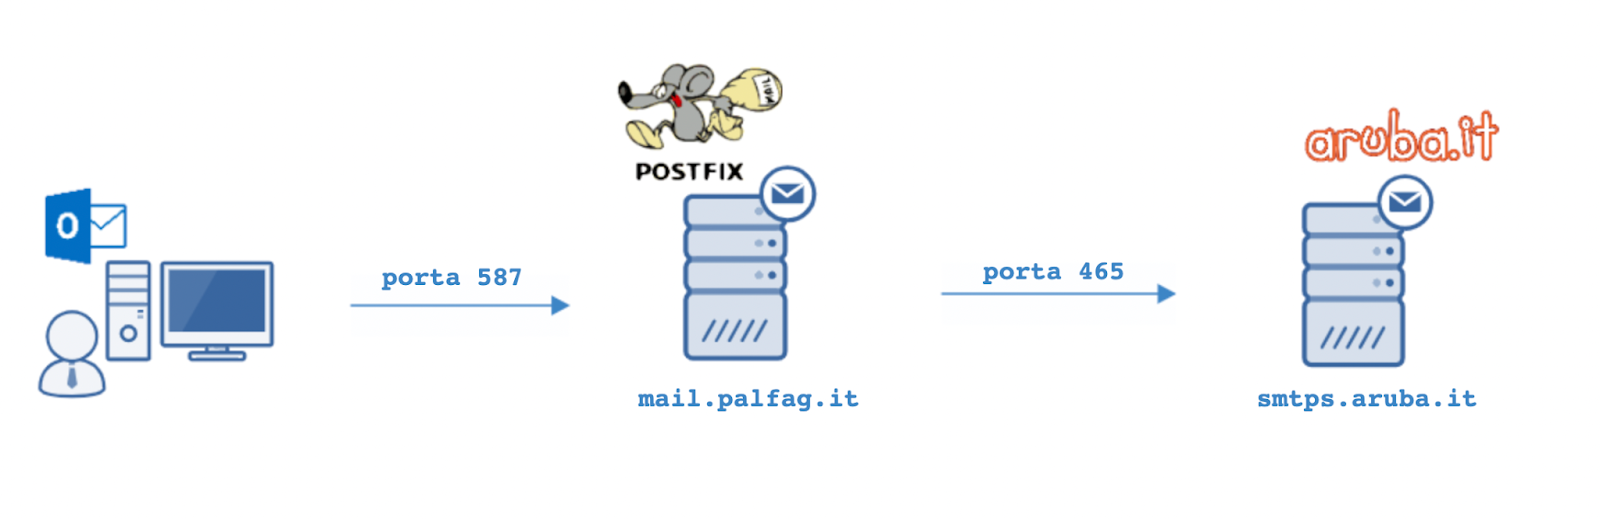
\includegraphics[width=12cm, height=20cm, keepaspectratio]{Screenshot 2021-05-03 at 11.28.07.png}
    \caption{Configurazione di Postfix}\label{confPostfix}
  \end{figure}

Innanzitutto sarà necessario installare i seguenti pacchetti:

\begin{verbatim}
    yum install postfix mailx cyrus-sasl cyrus-sasl-plain
\end{verbatim}


Creare un file, nel mio caso che ho chiamato \textit{sasl\_passwd} dove andremo a mettere le credenziali
necessarie per l'autenticazione presso il server Aruba:

\begin{verbatim}
    nano /etc/postfix/sasl_passwd
    [smtps.aruba.it]:465    paolo.fagioli@certimeter.it:pwd
\end{verbatim}

Processare il file contenente le credenziali:

\begin{verbatim}
    postmap /etc/postfix/sasl_passwd
\end{verbatim}

Editare il file \textit{/etc/postfix/main.cf}:

\begin{verbatim}
    myhostname = mail.palfag.it
    relayhost= [smtps.aruba.it]:465
    mynetworks = 192.168.8.0/24 127.0.0.0/8
    smpd_banner = $myhostname ESMTP $mail_name ($mail_version)
    mailbox_size_limit = 0
    inet_interfaces = all
    inet_protocols = all
    append_dot_mydomain = no
    readme_directory = no
\end{verbatim}

Sempre all'interno del file \textit{/etc/postfix/main.cf} inserire i parametri per la configurazione di TLS,
in questo momento saranno necessari i certificato e chiave generati precedentemente:

\begin{verbatim}
    # TLS parameters
    smtpd_tls_cert_file=/etc/pki/tls/certs/apache-selfsigned.crt
    smtpd_tls_key_file=/etc/pki/tls/private/apache-selfsigned.key

    smtpd_tls_security_level=encrypt
    smtp_tls_CApath=/etc/ssl/certs
    smtp_tls_security_level=encrypt
    smtp_tls_session_cache_database = btree:${data_directory}/smtp_scache
    smtp_sasl_password_maps = hash:/etc/postfix/sasl_passwd
    smtp_tls_wrappermode = yes
    smtp_use_tls = yes
    smtp_sasl_auth_enable = yes
    smtp_sasl_security_options = noanonymous
\end{verbatim}

Avviare Postfix:
\begin{verbatim}
    systemctl start postfix.service
\end{verbatim}

A questo punto possiamo verificare il corretto funzionamento della funzione di inoltro verso i server di Aruba 
provando ad inviare una email da terminale:

\begin{verbatim}
    echo corpo | mail -s “Oggetto” -r emailMittente emailDestinatario 
\end{verbatim}

Una volta testato il funzionamento, sarà necessario configurare Postfix in modo che ascolti dalle porte 465 e 587 
(la porta 25 è già configurata di default).

Editare il file \textit{/etc/postfix/master.cf}. Attraverso la seguente configurazione Postfix ascolterà 
sulla porta 587 e sarà dotato di tutte le impostazioni necessarie per supportare il protocollo TLS:

\begin{verbatim}
    submission inet n       -       n       -       -       smtpd
  -o syslog_name=postfix/submission
  -o smtpd_sasl_auth_enable=yes
  -o smtpd_sasl_security_options=noanonymous
  -o broken_sasl_auth_clients=yes
  -o smtpd_tls_security_level=encrypt
  -o smtpd_tls_key_file=/etc/pki/tls/private/apache-selfsigned.key
  -o smtpd_tls_cert_file=/etc/pki/tls/certs/apache-selfsigned.crt
  -o smtpd_tls_loglevel=1
  -o smtpd_tls_session_cache_timeout=3600s
  -o smtpd_tls_session_cache_database=btree:/var/lib/postfix/smtpd_tls_cache
  -o tls_random_source=dev:/dev/urandom
  -o tls_random_exchange_name=/var/lib/postfix/prng_exch
  -o smtpd_tls_auth_only=yes
  -o smtpd_recipient_restrictions=permit_sasl_authenticated,reject
  -o smtpd_relay_restrictions=permit_sasl_authenticated,reject
\end{verbatim}

Un procedimento simile per fare in modo che ascolti anche dalla porta 465:

\begin{verbatim}
    smtps     inet  n       -       n       -       -       smtpd
    -o syslog_name=postfix/smtps
    -o smtpd_sasl_auth_enable=yes
    -o smtpd_sasl_security_options=noanonymous
    -o broken_sasl_auth_clients=yes
    -o smtpd_recipient_restrictions=permit_sasl_authenticated,reject
    -o smtpd_tls_security_level=encryptà
    -o smtpd_tls_wrappermode=yes
    -o smtpd_tls_key_file=/etc/pki/tls/private/apache-selfsigned.key
    -o smtpd_tls_cert_file=/etc/pki/tls/certs/apache-selfsigned.crt
    -o smtpd_tls_loglevel=1
    -o smtpd_tls_session_cache_timeout=3600s
    -o smtpd_tls_session_cache_database=btree:/var/lib/postfix/smtpd_tls_cache
    -o tls_random_source=dev:/dev/urandom
    -o tls_random_exchange_name=/var/lib/postfix/prng_exch
    -o smtpd_tls_auth_only=yes
\end{verbatim}

Avviare sasl\_authd
\begin{verbatim}
    systemctl start sasl\_authd.services
\end{verbatim}

Riavviare Postfix
\begin{verbatim}
    systemctl restart postfix.service
\end{verbatim}

Da questo momento Postfix è pronto per svolgere il suo lavoro.